\begin{figure}[tbp]
\centering
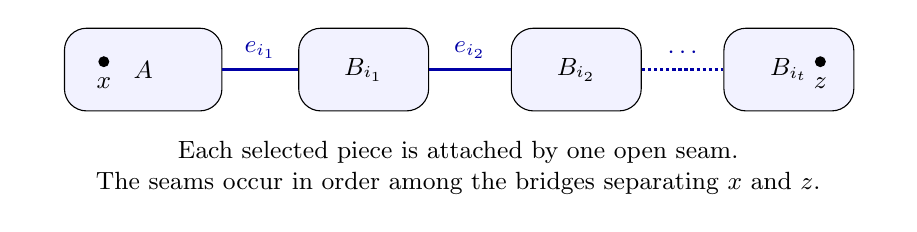
\begin{tikzpicture}[x=1cm,y=1cm,font=\small,
  piece/.style={draw,rounded corners=8pt,fill=blue!5,minimum width=1.65cm,minimum height=1.05cm},
  seam/.style={very thick,blue!65!black},dot/.style={circle,fill,inner sep=1.4pt}]
\node[piece,minimum width=2cm] (a) at (0.3,0) {$A$};
\node[piece] (b1) at (3.1,0) {$B_{i_1}$};
\node[piece] (b2) at (5.8,0) {$B_{i_2}$};
\node[piece] (bt) at (8.5,0) {$B_{i_t}$};
\draw[seam] (a.east)--node[above] {$e_{i_1}$} (b1.west);
\draw[seam] (b1.east)--node[above] {$e_{i_2}$} (b2.west);
\draw[seam,densely dotted] (b2.east)--node[above] {$\cdots$} (bt.west);
\node[dot,label=below:$x$] at (-0.2,0.10) {};
\node[dot,label=below:$z$] at (8.9,0.10) {};
\node[align=center,text width=10.7cm] at (4.3,-1.25)
{Each selected piece is attached by one open seam.\\
The seams occur in order among the bridges separating $x$ and $z$.};
\end{tikzpicture}
\caption{The chain produced by the switching procedure. Cutting the
selected seams recovers the inserted pieces and the initial cluster
$A$. The drawing shows vertex sets and selected open seams, with
internal edges and other incident edges omitted.}
\label{fig:splicing}
\end{figure}
